\section{Resultados}

Nos testes foram utiliza dois modelos de árvore tree2D\_Nterm128.vtk e tree3D\_Nterm016.vtk.

\subsection{Leitura e representação do modelo}
A Tabela~\ref{tab:modelo} resume o modelo utilizado nos testes e a Figura ~\ref{fig:comparacao_arvores} mostra as árvore representadas por tubos.

\begin{table}[!h]
  \centering\small
  \caption{Características do modelo CCO utilizado.}
  \label{tab:modelo}
  \begin{tabular}{ll}
    \toprule
    \textbf{Atributo} & \textbf{Valor}\\
    \midrule
    Arquivo & tree2D\_Nterm128.vtk\\
    Dimensão & 2D\\
    Número de pontos & 256\\
    Número de segmentos & 255\\
    Raio mínimo & 0.1454243\\
    Raio máximo & 1.1929671\\
    \bottomrule
  \end{tabular}
\end{table}

\begin{figure}[H]
    \centering
    % --- Primeira linha ---
    \begin{subfigure}{0.48\textwidth}
        \centering
        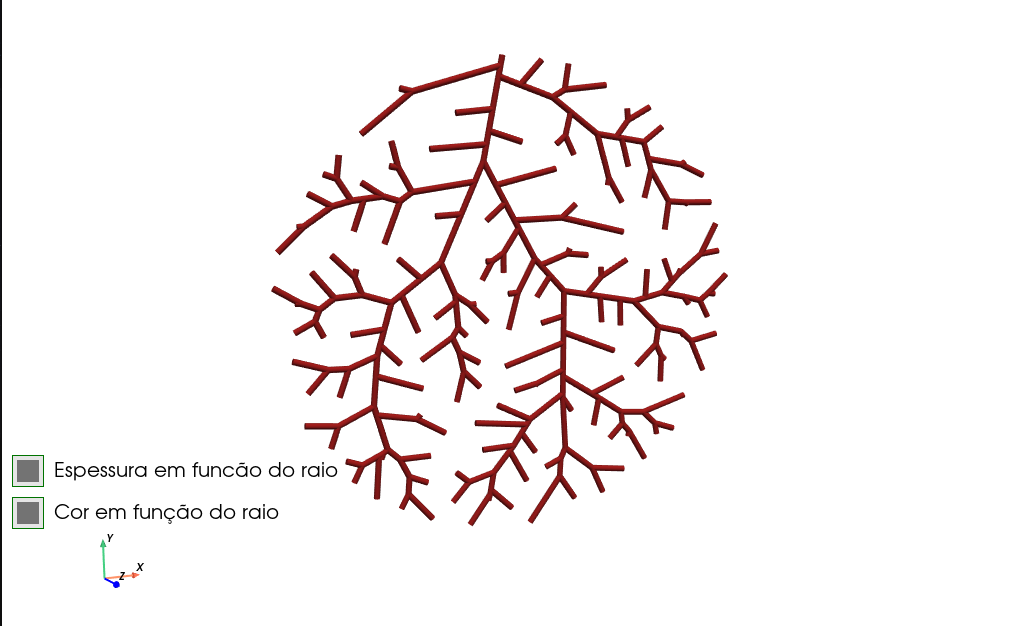
\includegraphics[width=\linewidth]{figures/desligado.png}
        \caption{Árvore com espessura desligada.}
        \label{fig:espessura}
    \end{subfigure}
    \hfill % Adiciona espaço horizontal entre as duas figuras
    \begin{subfigure}{0.48\textwidth}
        \centering
        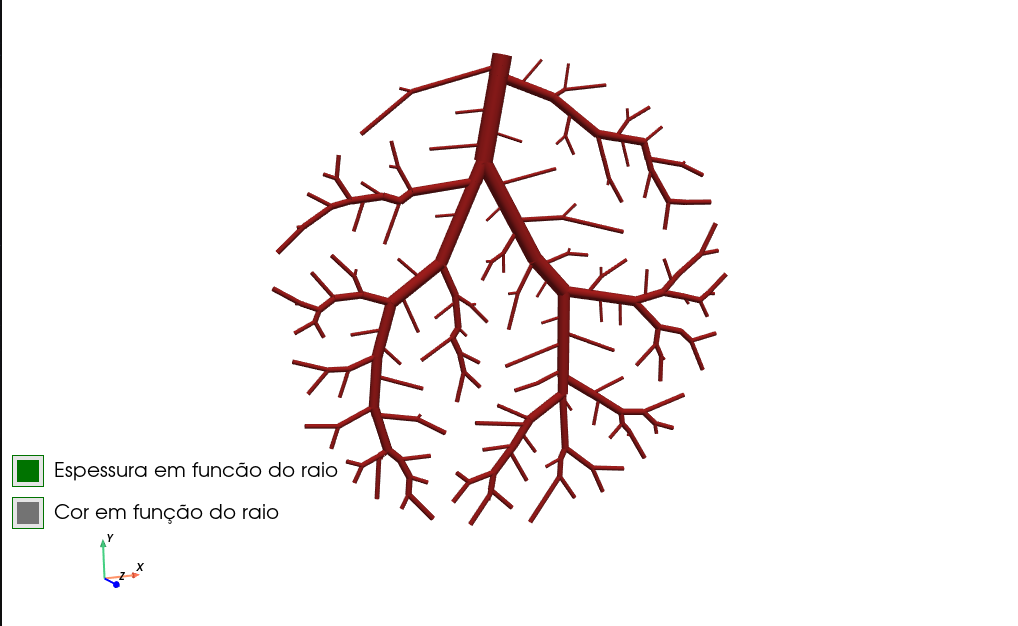
\includegraphics[width=\linewidth]{figures/espessura.png}
        \caption{Árvore com espessura relacionada ao raio.}
        \label{fig:espessura_raio}
    \end{subfigure}

    \vspace{1em} % Espaço vertical entre a primeira e a segunda linha

    % --- Segunda linha ---
    \begin{subfigure}{0.48\textwidth}
        \centering
        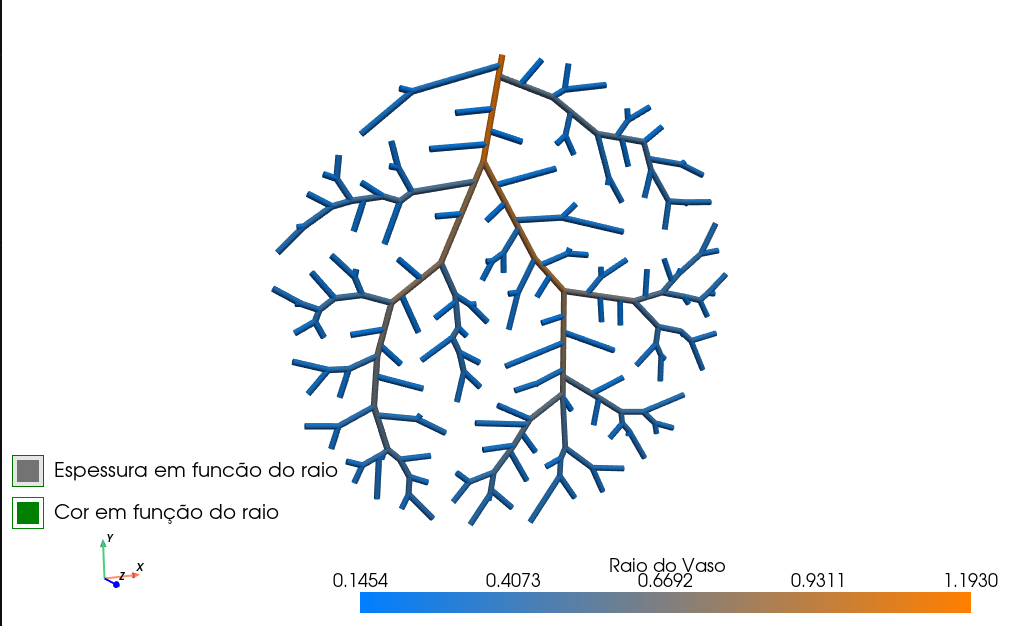
\includegraphics[width=\linewidth]{figures/cor.png}
        \caption{Árvore com espessura relacionada com a cor.}
        \label{fig:espessura_cor}
    \end{subfigure}
    \hfill
    \begin{subfigure}{0.48\textwidth}
        \centering
        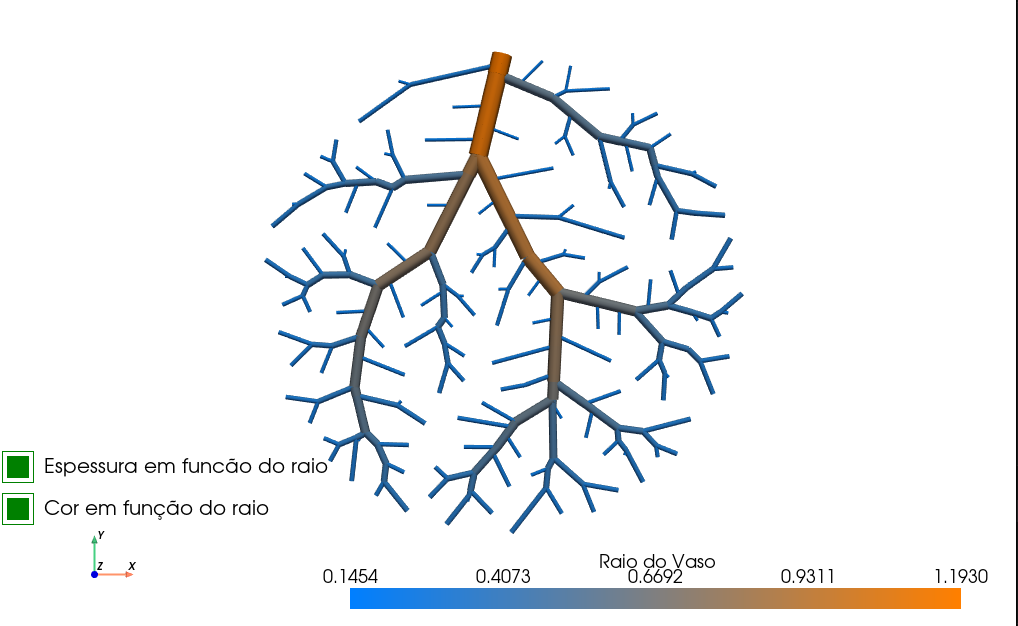
\includegraphics[width=\linewidth]{figures/cor_espessura.png}
        \caption{Árvore com espessura relacionada à cor e ao raio.}
        \label{fig:cor_raio}
    \end{subfigure}

    \caption{Comparação das diferentes configurações da árvore.}
    \label{fig:comparacao_arvores}
\end{figure}

\subsection{Modelo utilizado e atributos}

O modelo de exemplo é \texttt{tree3D\_Nterm016.vtk}. A leitura direta do arquivo e a informação apresentada pela aplicação indicam 32 pontos e 31 células lineares. O atributo \texttt{raio} possui mínimo de 0,2261241 e máximo de 0,6870107. Esses valores são reproduzidos na interface durante a execução (Figura~\ref{fig:app}).

\begin{figure}[H]
\centering
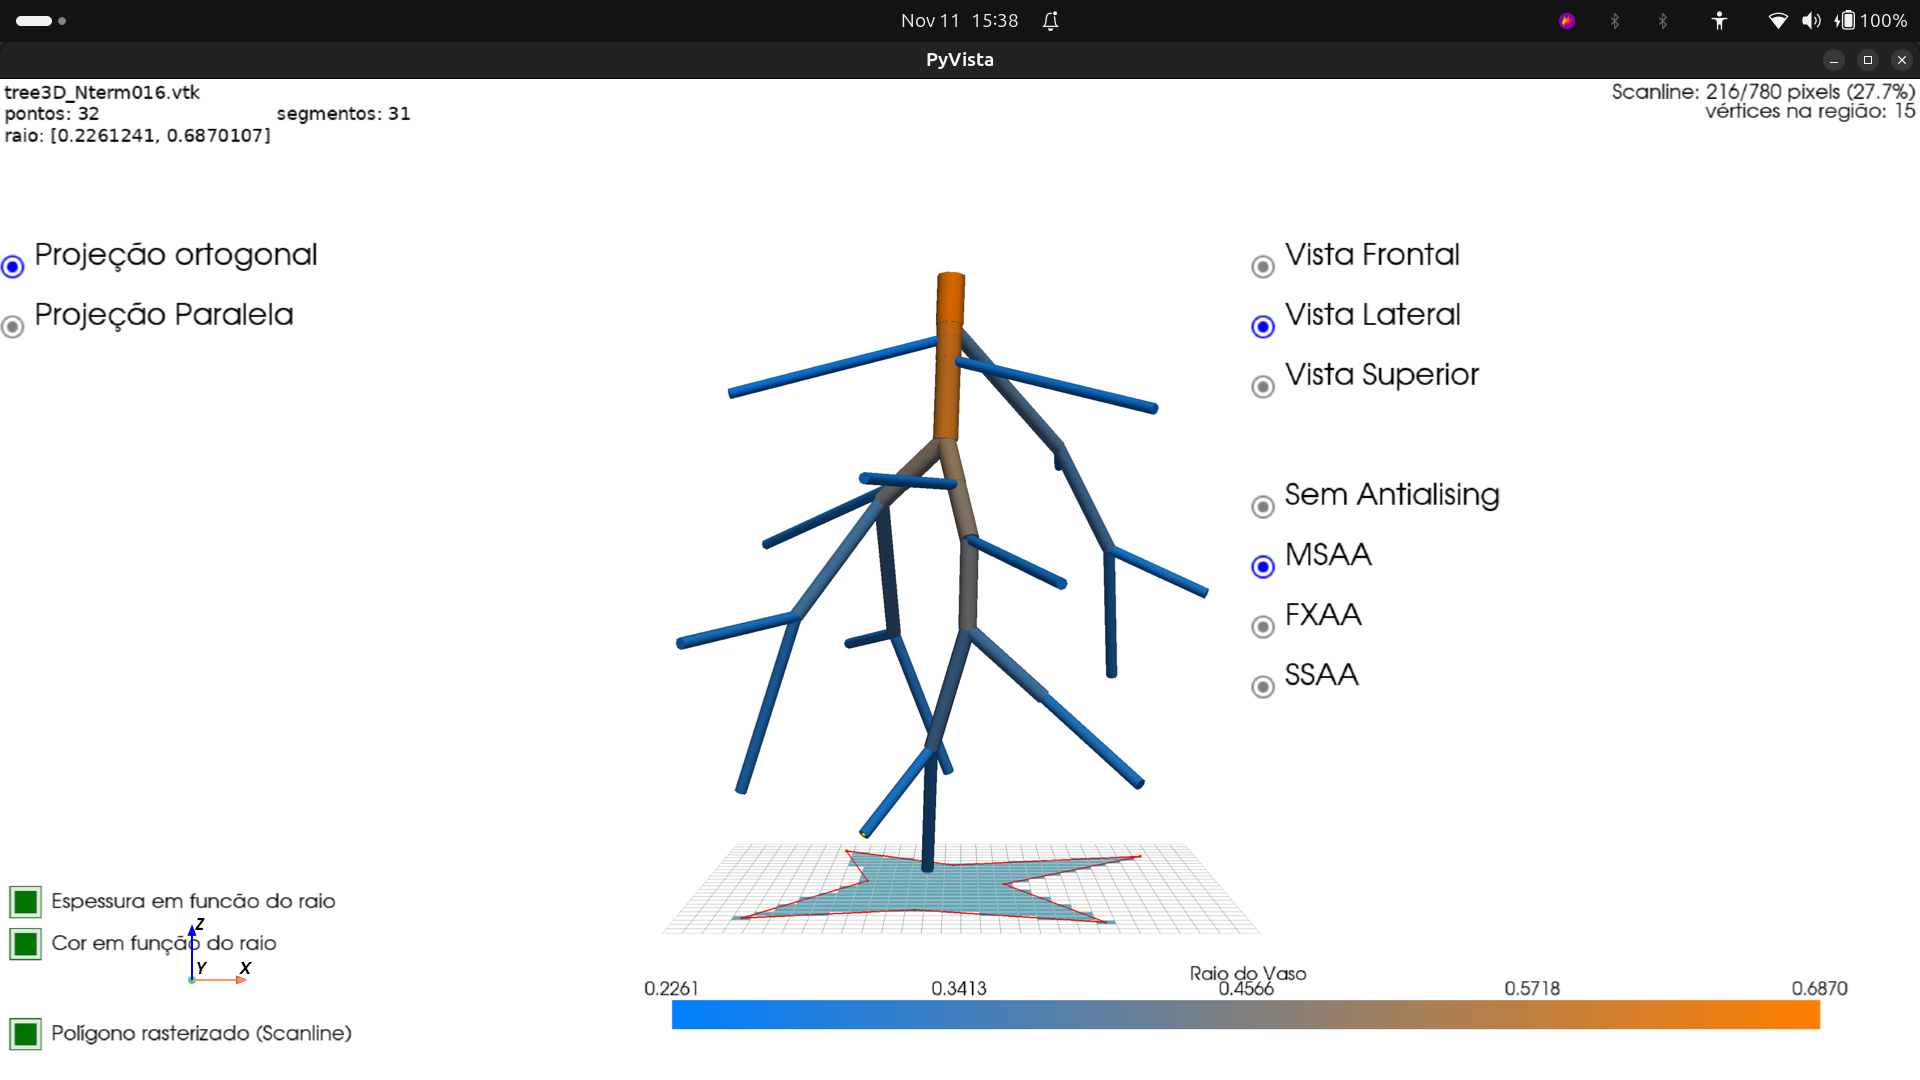
\includegraphics[width=0.94\textwidth]{figures/aplicacao_modelo_3d.png}
\caption{Aplicação em execução com o modelo \texttt{tree3D\_Nterm016.vtk}, mostrando os dados de entrada, a árvore tubular, os controles de câmera, antialiasing e atributos visuais.}
\label{fig:app}
\end{figure}

A Figura~\ref{fig:refcomp} compara a imagem de referência fornecida pelo docente para o mesmo conjunto com uma captura da aplicação. A comparação é qualitativa: ambas apresentam a estrutura ramificada, mas a aplicação adiciona controles interativos e a codificação visual pelo atributo de raio.

\begin{figure}[H]
\centering
\begin{subfigure}[t]{0.38\textwidth}
\centering
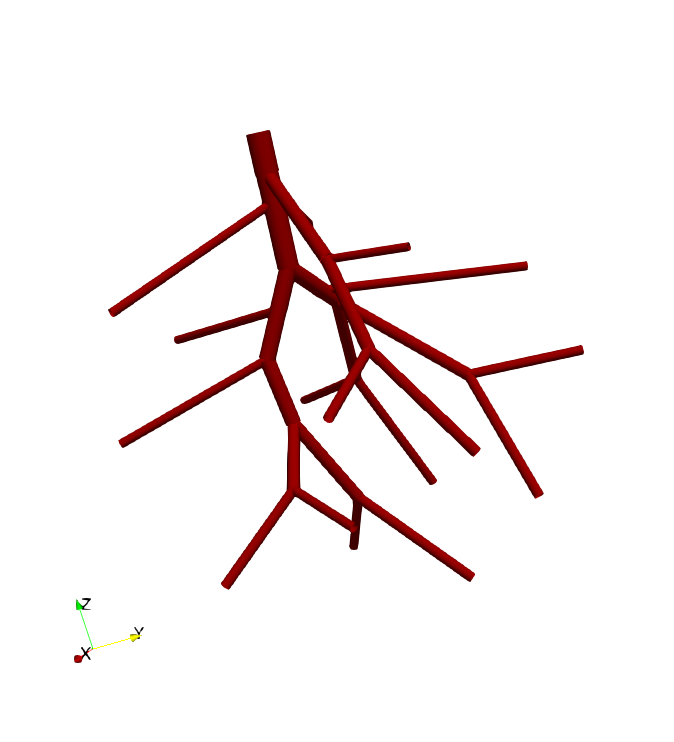
\includegraphics[height=5.4cm,keepaspectratio]{figures/tree3D_Nterm016_tube_solid.png}
\caption{Imagem de referência do docente.}
\end{subfigure}\hfill
\begin{subfigure}[t]{0.58\textwidth}
\centering
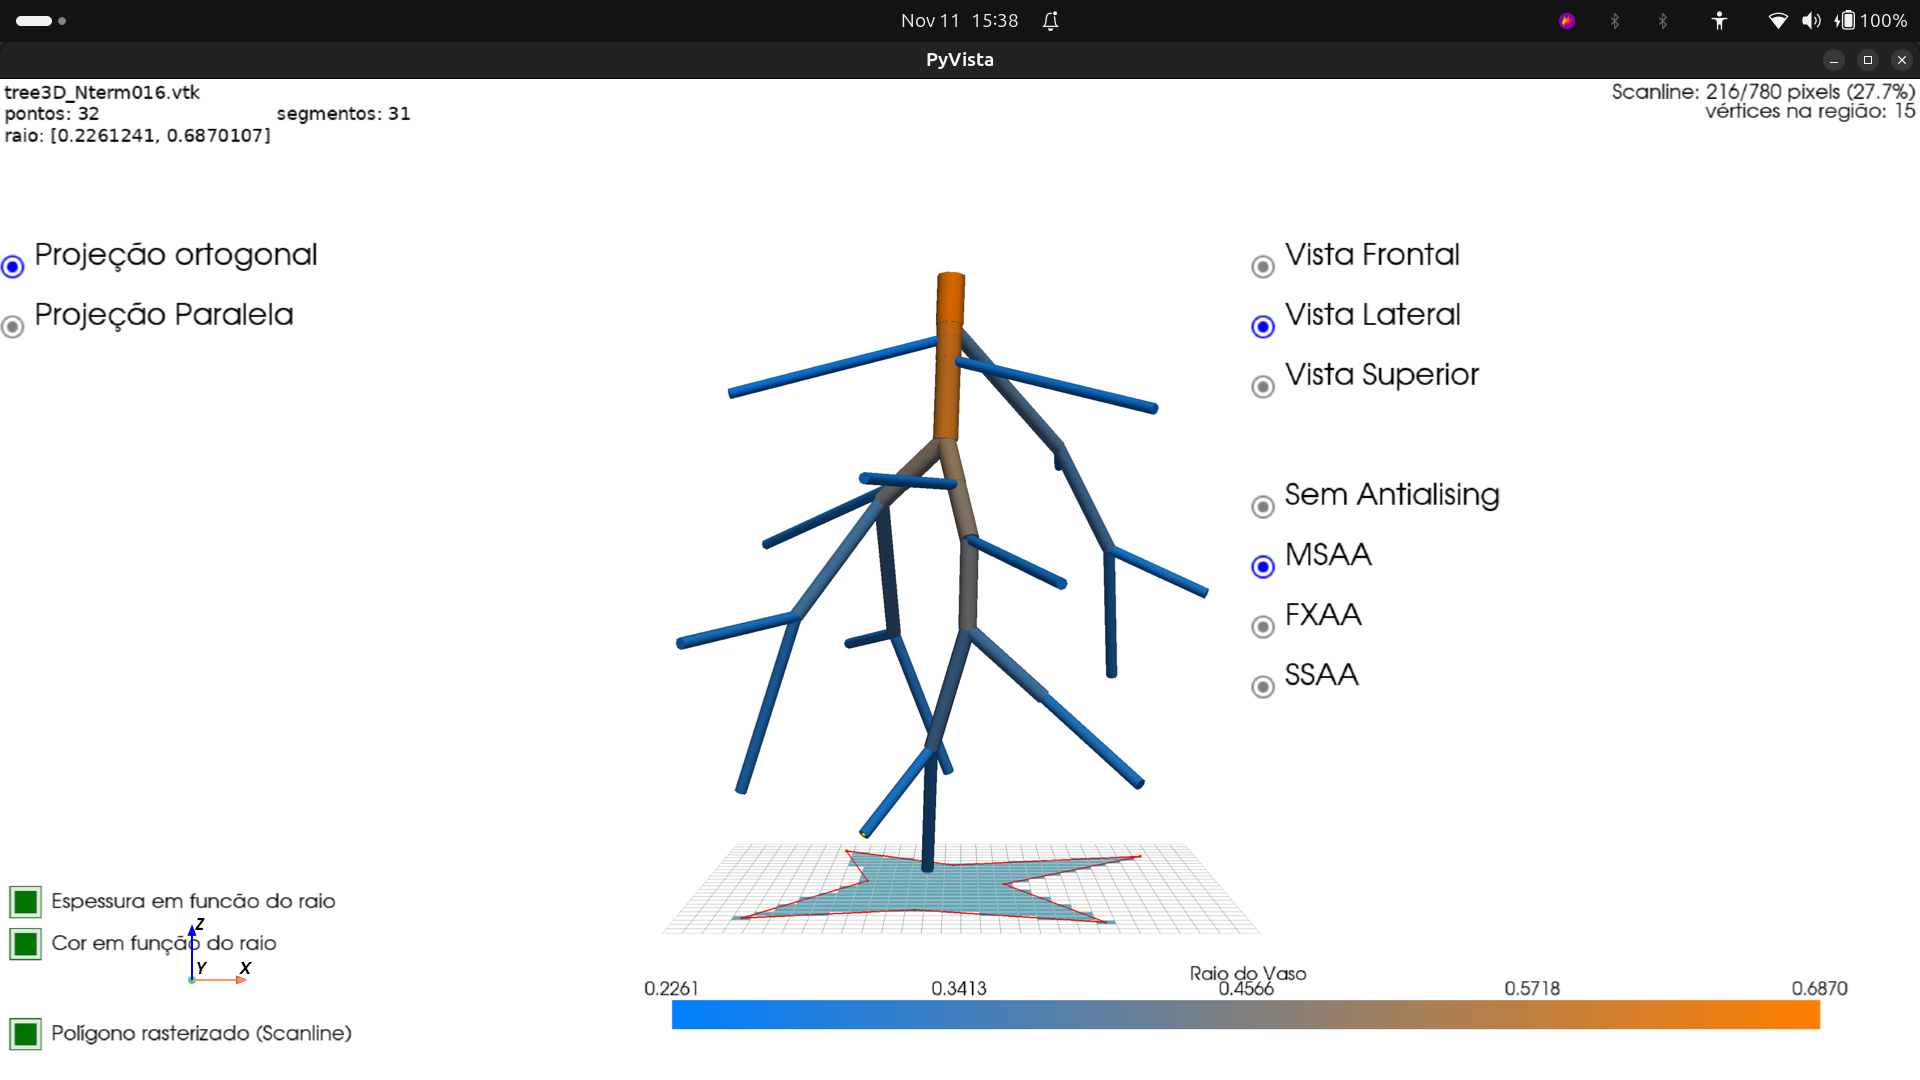
\includegraphics[width=\textwidth]{figures/aplicacao_modelo_3d.png}
\caption{Visualização produzida pela aplicação.}
\end{subfigure}
\caption{Comparação qualitativa do modelo tridimensional com a referência disponibilizada.}
\label{fig:refcomp}
\end{figure}

Na Figura \ref{fig:comparacao_vista} mostra a comparação da visualização da árvore ao mudar a câmera de posição.

\begin{figure}[H]
    \centering
    % --- Primeira linha ---
    \begin{subfigure}{0.48\textwidth}
        \centering
        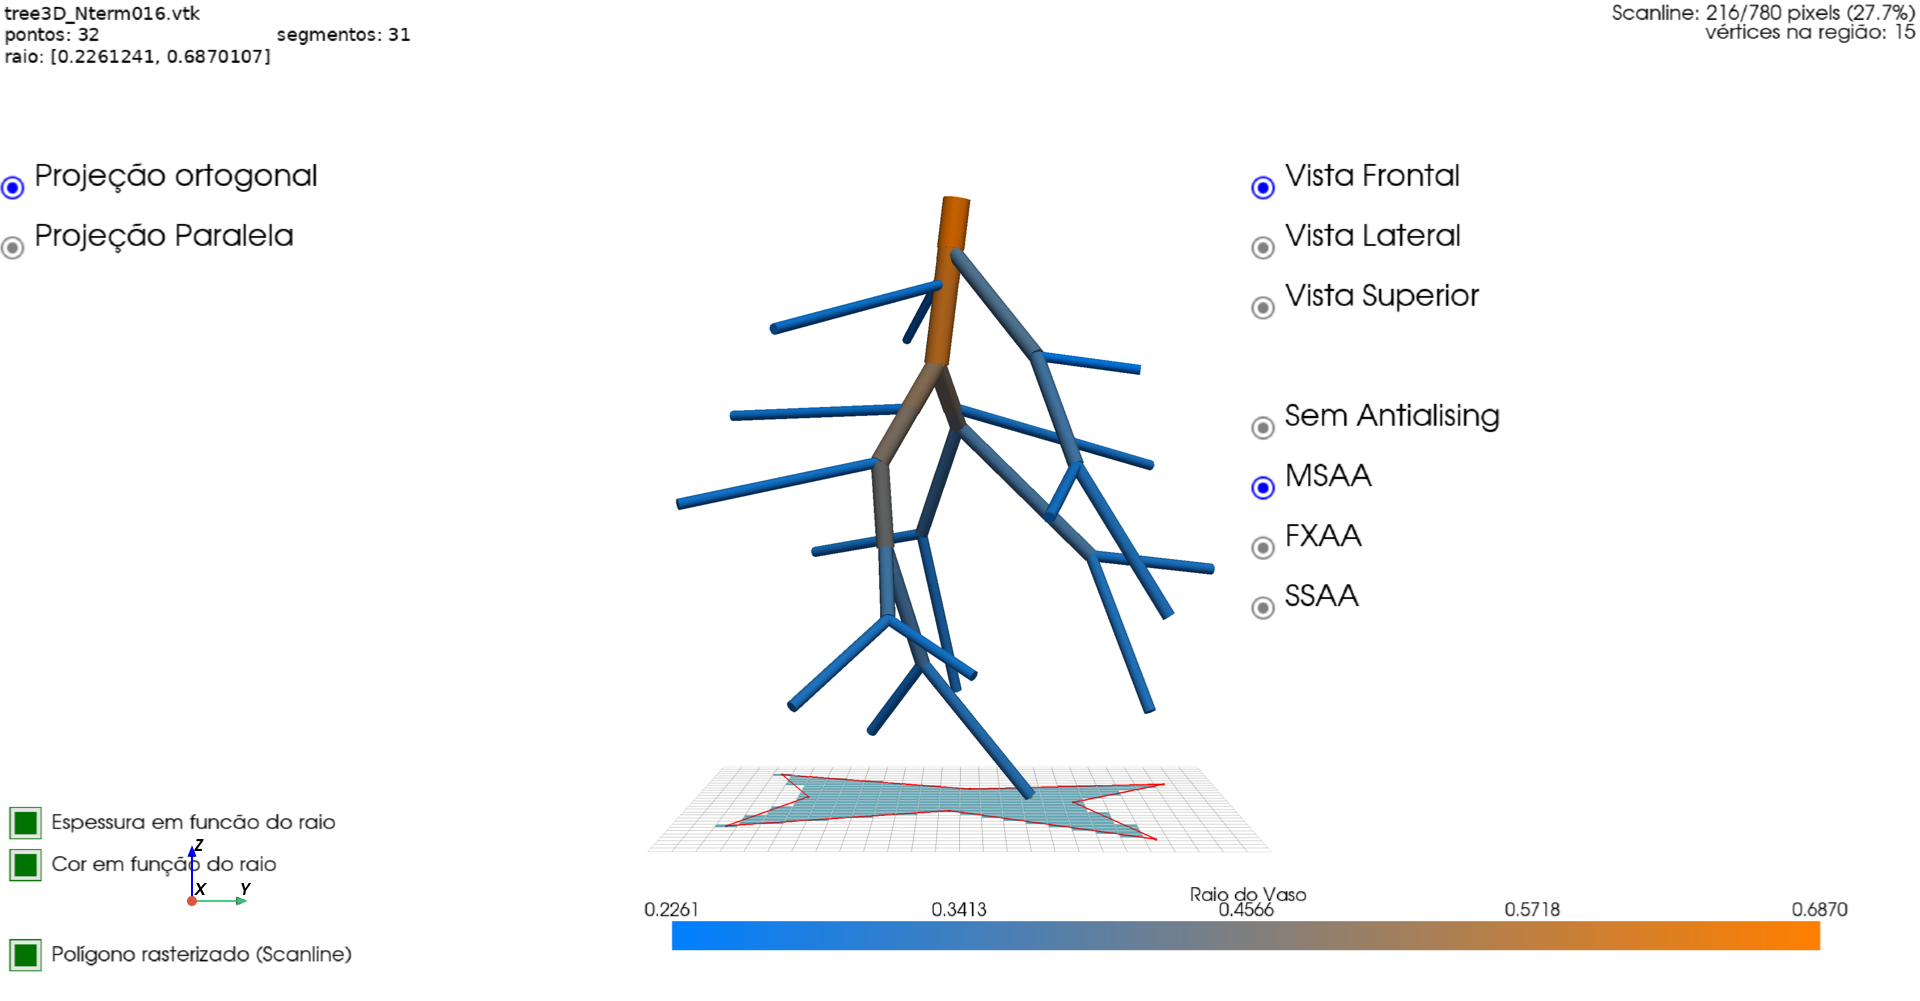
\includegraphics[width=\linewidth]{figures/vista_frontal.png}
        \caption{Frontal.}
        \label{fig:frontal}
    \end{subfigure}
    \hfill % Adiciona espaço horizontal entre as duas figuras
    \begin{subfigure}{0.48\textwidth}
        \centering
        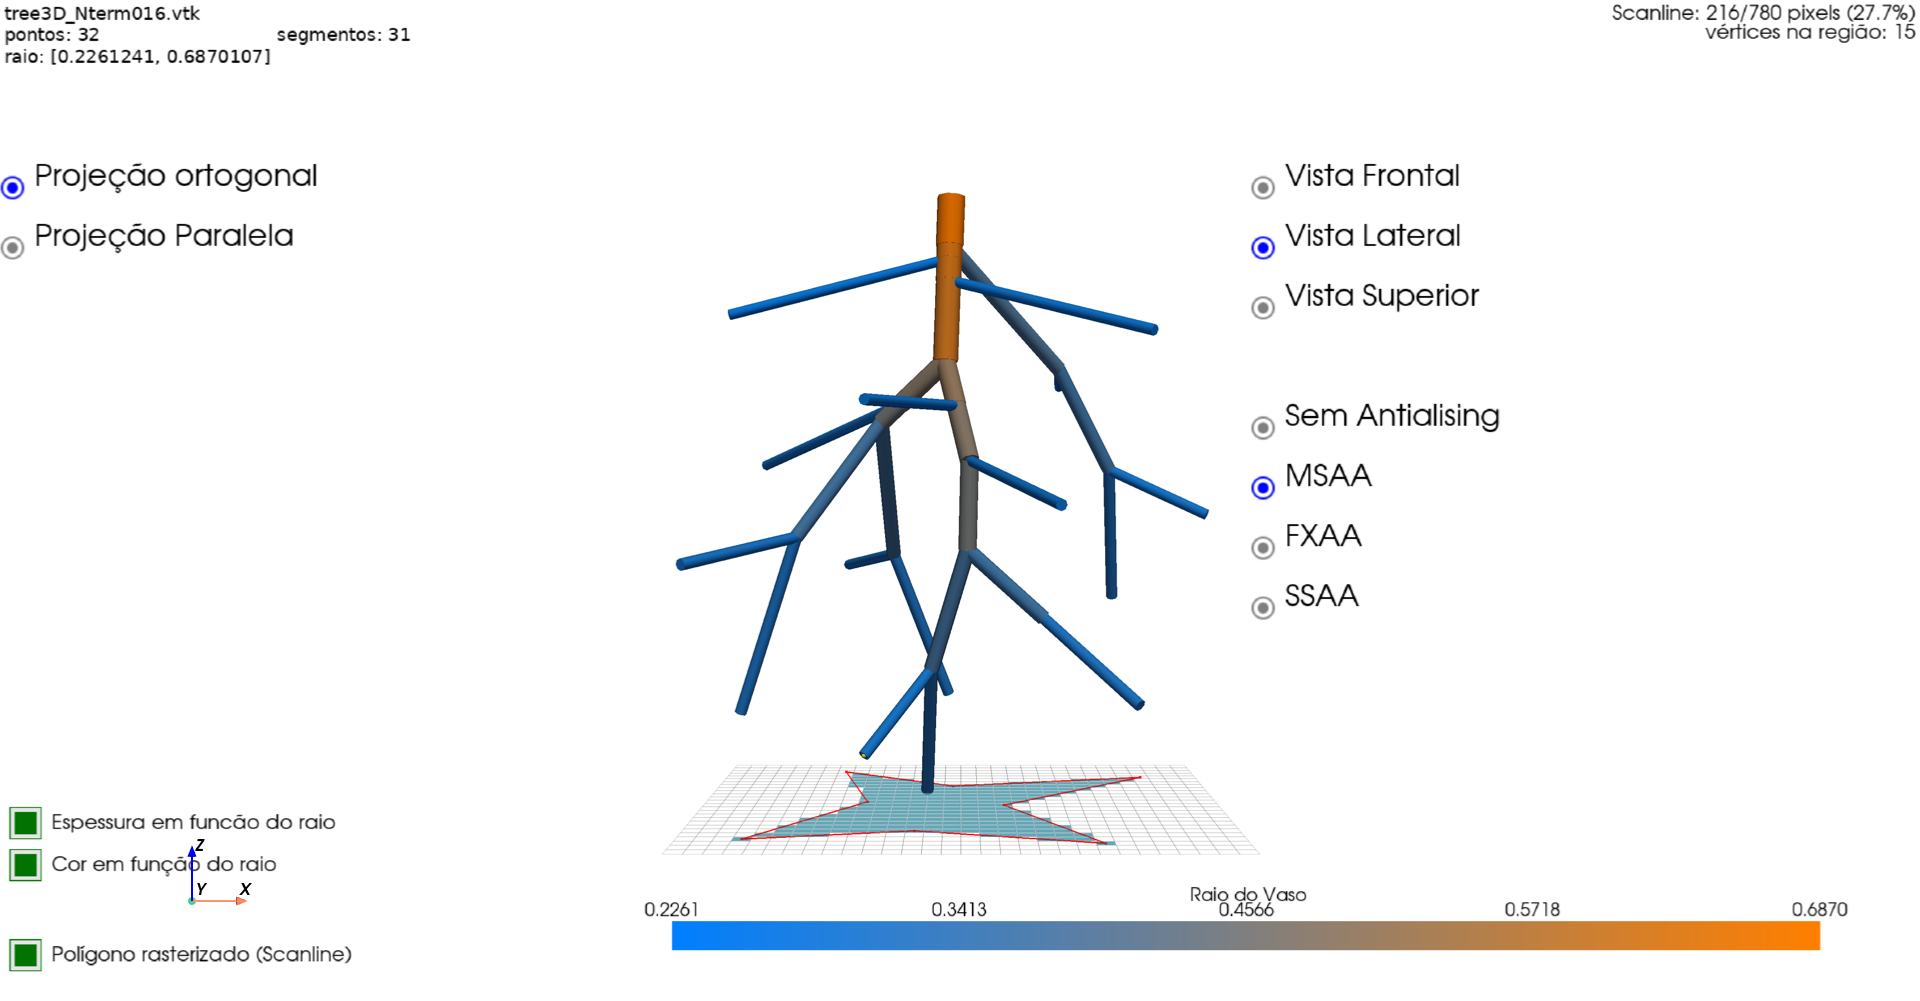
\includegraphics[width=\linewidth]{figures/vista_lateral.png}
        \caption{Lateral.}
        \label{fig:lateral}
    \end{subfigure}

    \vspace{1em} % Espaço vertical entre a primeira e a segunda linha

    % --- Segunda linha ---
    \begin{subfigure}{0.48\textwidth}
        \centering
        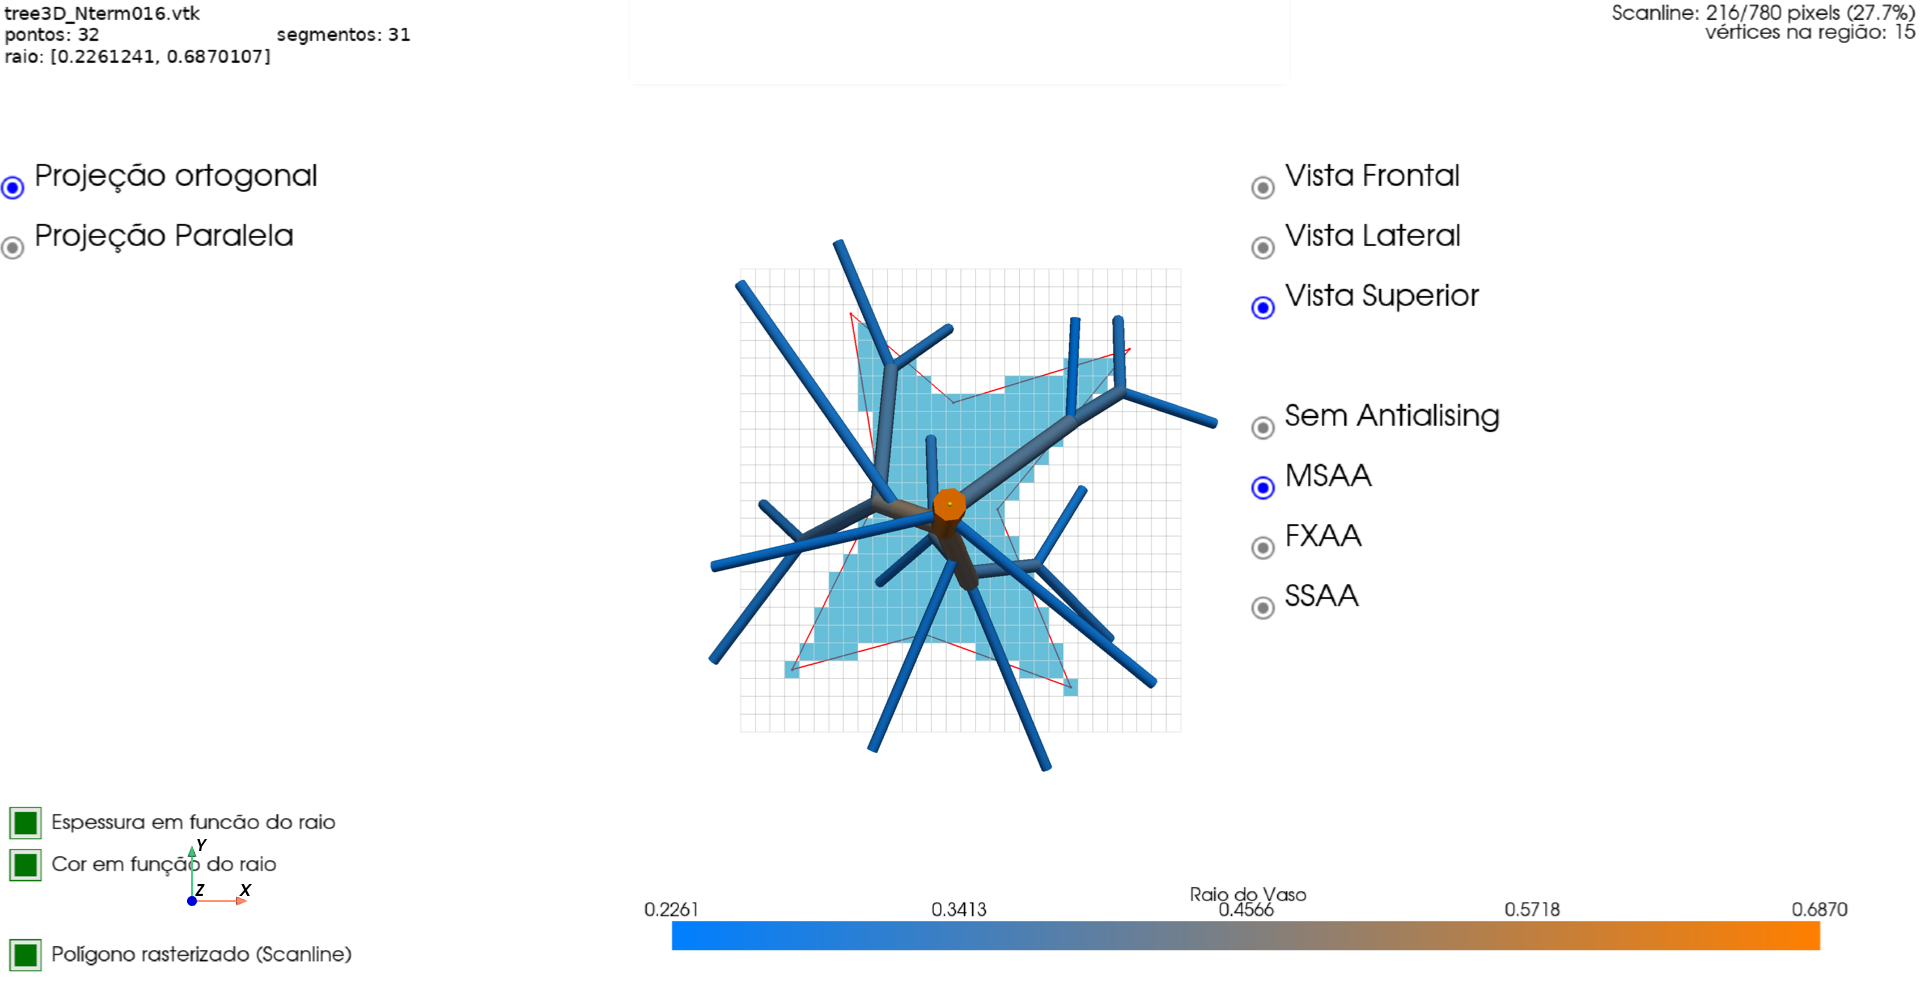
\includegraphics[width=\linewidth]{figures/vista_superior.png}
        \caption{Superior.}
        \label{fig:superior}
    \end{subfigure}

    \caption{Comparação da visualização da árvore ao mudar a posição da câmera.}
    \label{fig:comparacao_vista}
\end{figure}


\subsection{Rasterização de linhas}

Na Figura \ref{fig:rasterizacaoLinha} mostra a imagem gerada pela execução do algoritmo de Rasterização de Linha DDA e Bresenham.
\begin{figure}[H]
    \centering
    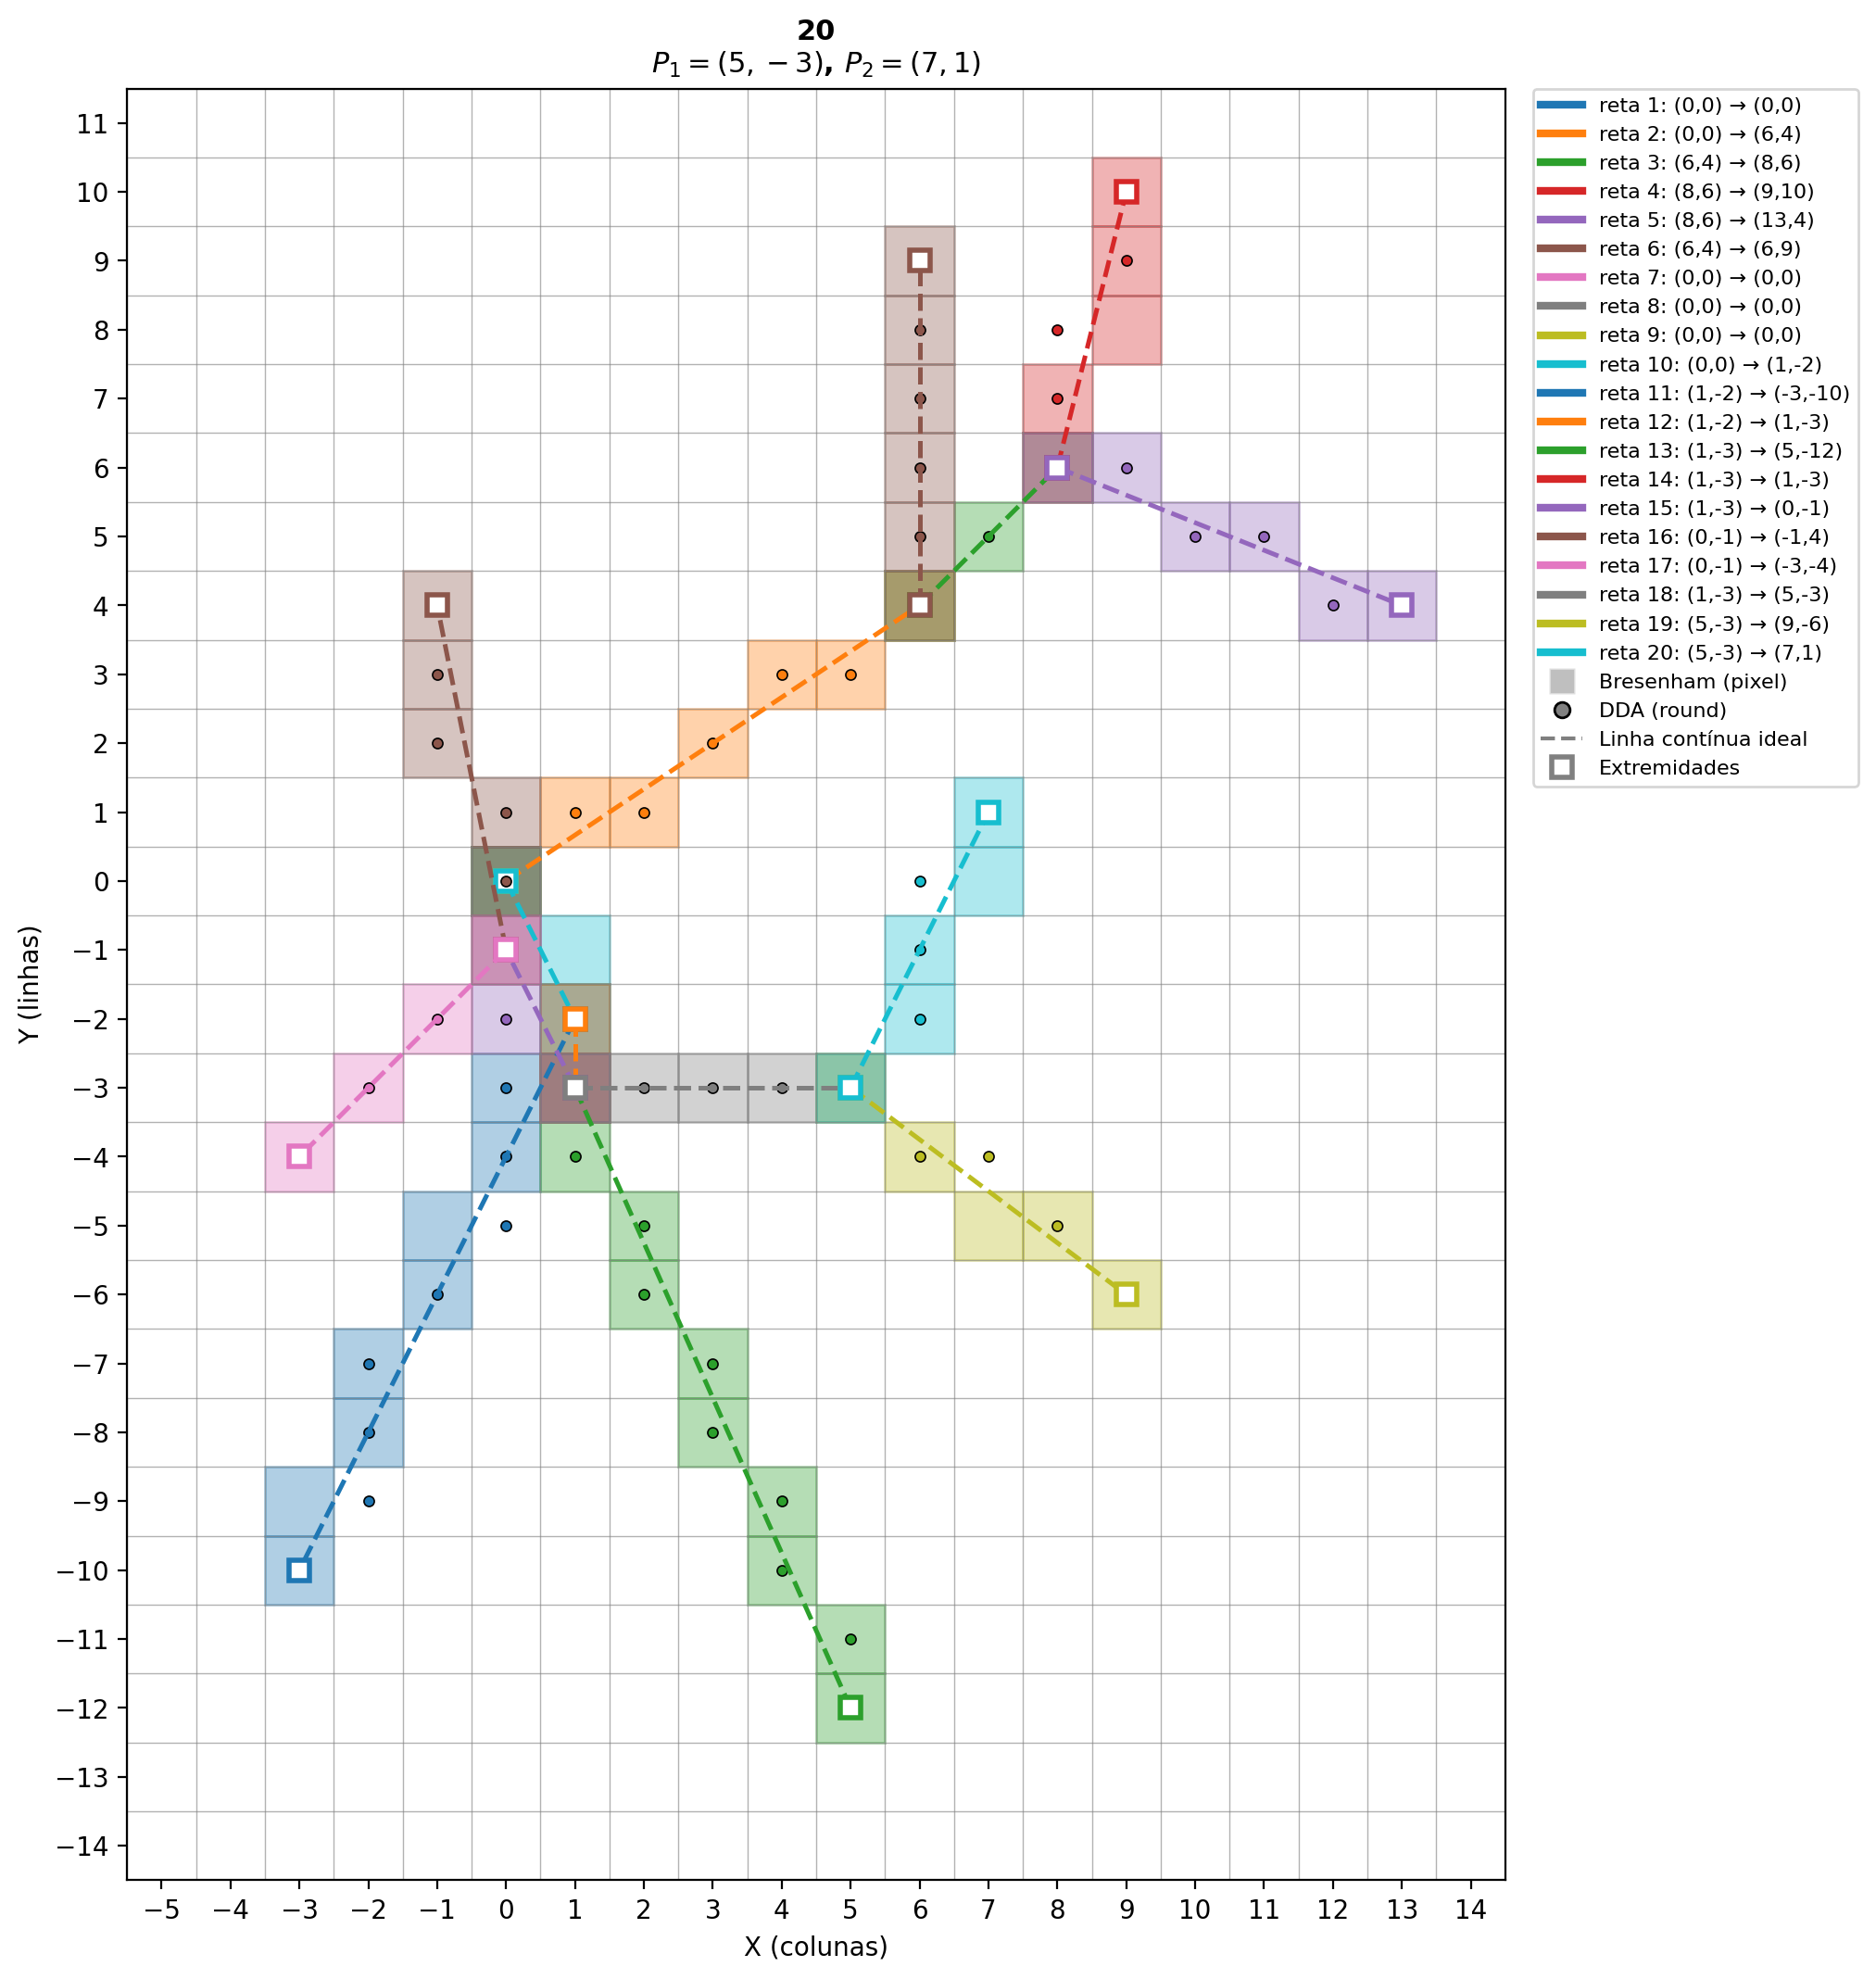
\includegraphics[width=1.0\linewidth]{figures/rasterizacao_linhas.png}
    \caption{Rasterização de Linhas.}
    \label{fig:rasterizacaoLinha}
\end{figure}

\subsection{Rasterização de polígonos}
Na Figura \ref{fig:comparacao_arvores_rasterizacao} mostra a comparação da rasterização de polígono (algoritmo Scanline) da árvore em dimensões diferentes do modelo do arquivo treexD\_Nterm128.vtk. A árvore a direita em azul é a árvore rasterizada.
\begin{figure}[H]
    \centering
    \begin{subfigure}{0.48\textwidth}
        \centering
        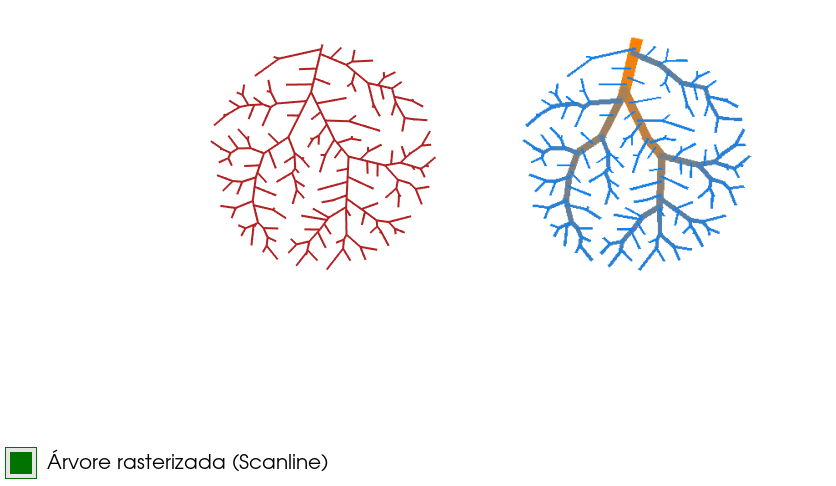
\includegraphics[width=\linewidth]{figures/rasterizacaoPligono_2D.png}
        \caption{Rasterização de Polígono em Árvore 2D.}
        \label{fig:rasteriza2D}
    \end{subfigure}
    \hfill % Adiciona espaço horizontal entre as duas figuras
    \begin{subfigure}{0.48\textwidth}
        \centering
        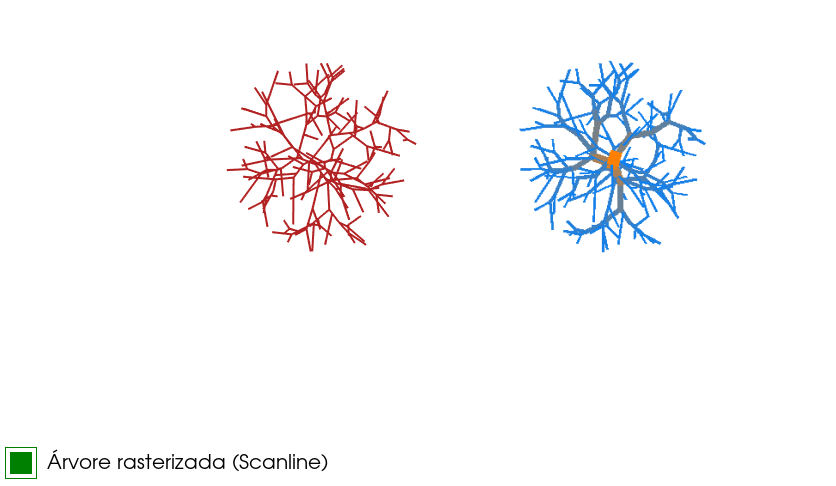
\includegraphics[width=\linewidth]{figures/rasterizacaoPoligono_3D.png}
        \caption{Rasterização de Polígono em Árvore 3D.}
        \label{fig:rasteriza3D}
    \end{subfigure}

    \caption{Comparação de Rasterização em diferentes dimensões de árvore.}
    \label{fig:comparacao_arvores_rasterizacao}
\end{figure}

\subsection{Antialiasing}
Na figura \ref{fig:comparacao_arvores_antiliasing} mostra a alternância entre ausência de antialiasing, MSAA, FXAA e SSAA.

\begin{figure}[H]
    \centering
    % --- Primeira linha ---
    \begin{subfigure}{0.48\textwidth}
        \centering
        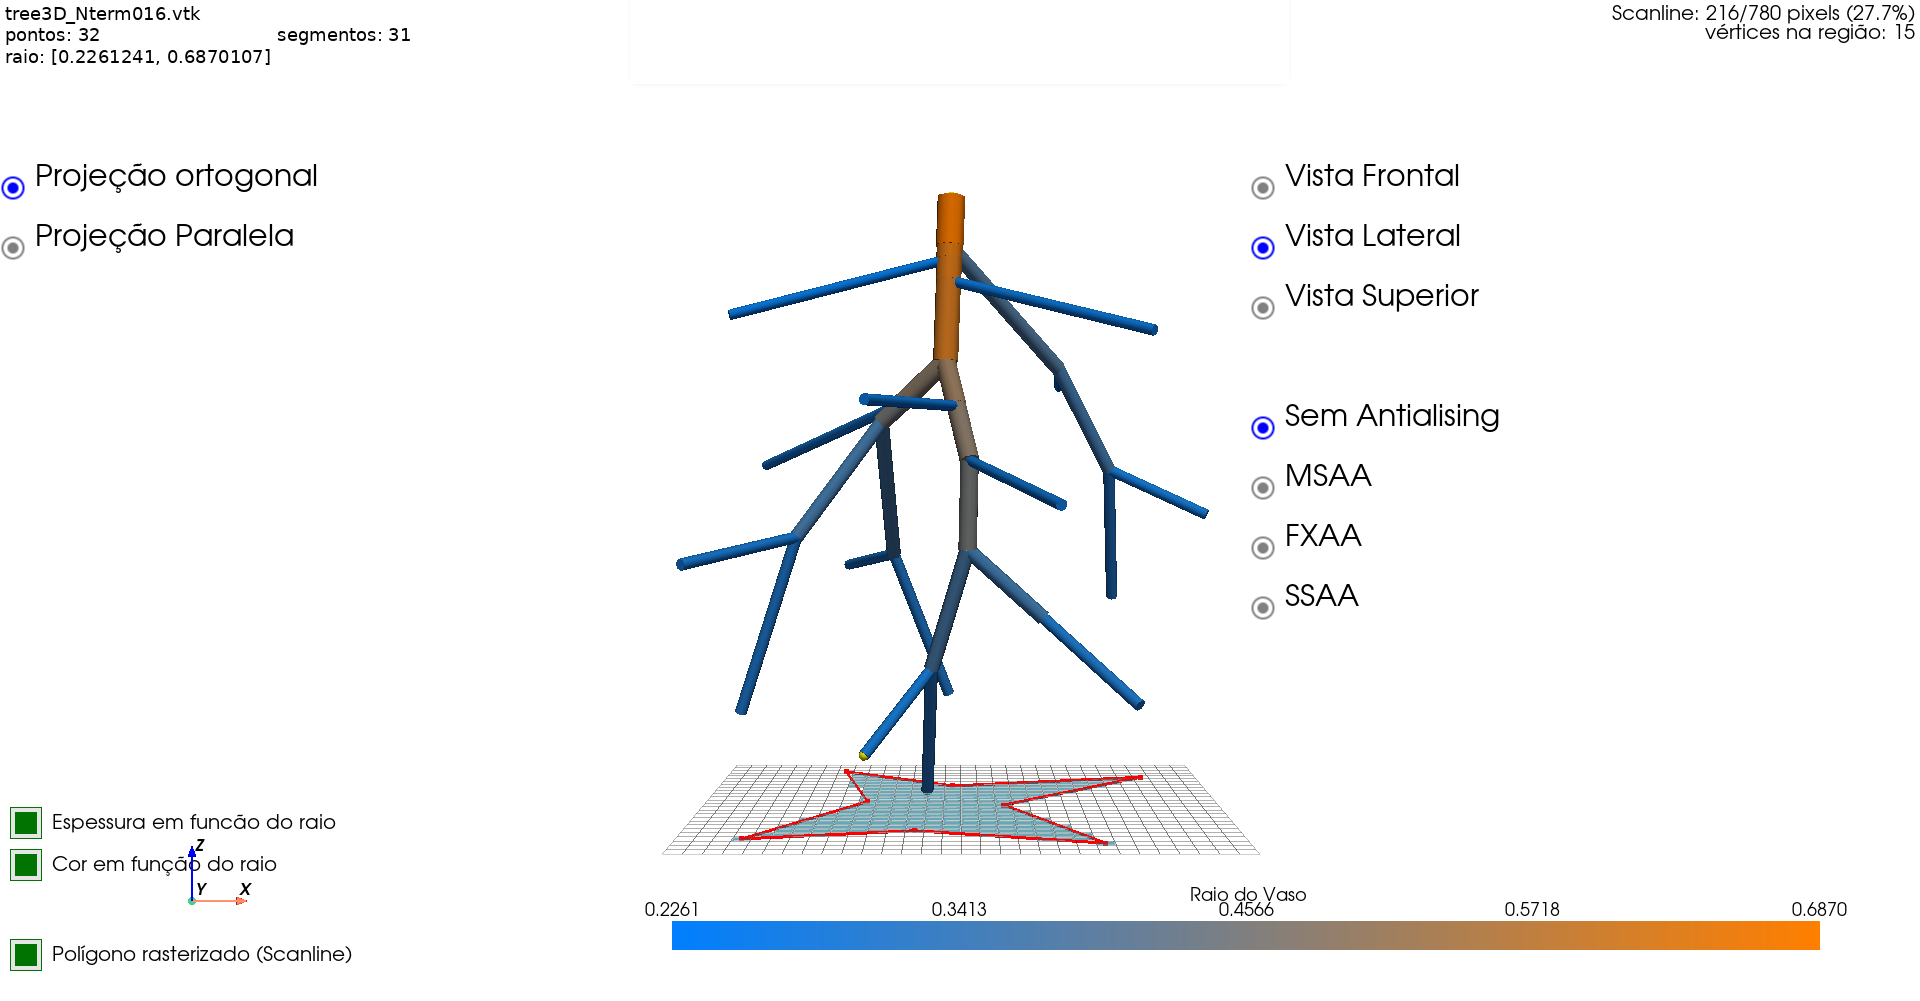
\includegraphics[width=\linewidth]{figures/aa_sem.png}
        \caption{Sem antialiasing}
        \label{fig:sem_antialiasing}
    \end{subfigure}
    \hfill % Adiciona espaço horizontal entre as duas figuras
    \begin{subfigure}{0.48\textwidth}
        \centering
        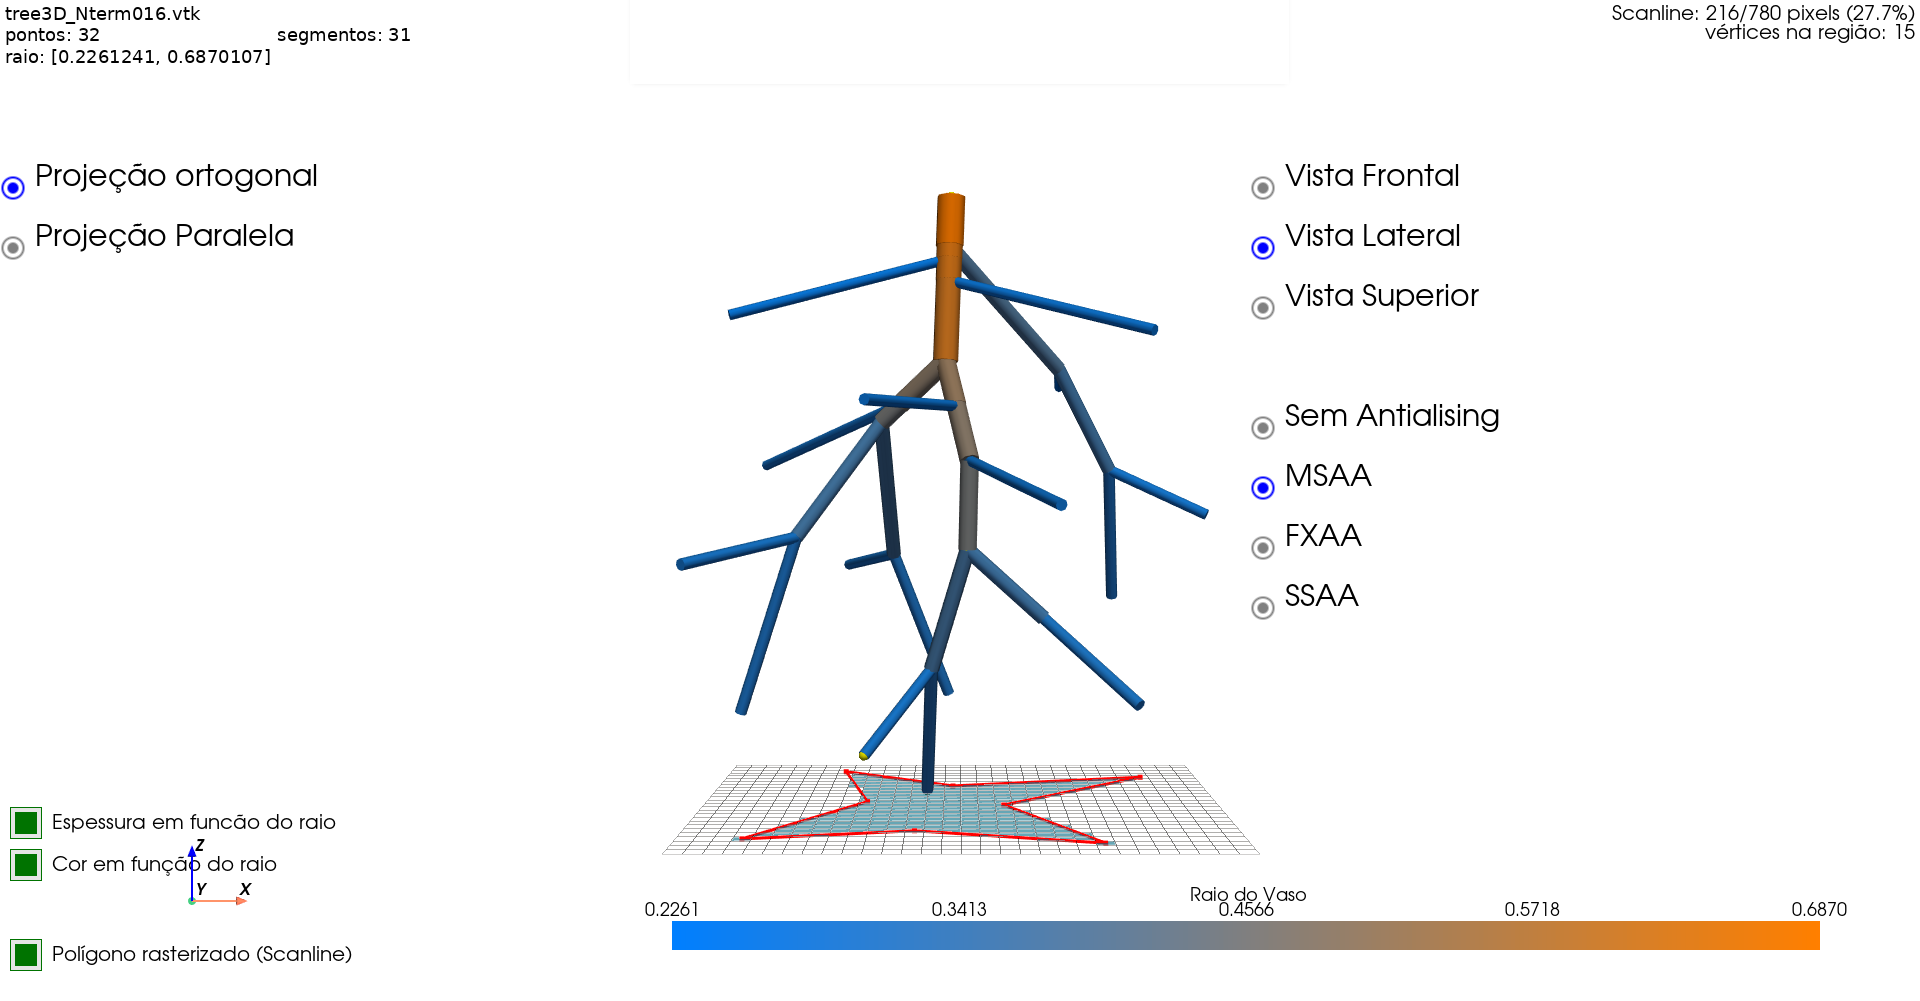
\includegraphics[width=\linewidth]{figures/aa_msaa.png}
        \caption{MSAA.}
        \label{fig:msaa}
    \end{subfigure}

    \vspace{1em} % Espaço vertical entre a primeira e a segunda linha

    % --- Segunda linha ---
    \begin{subfigure}{0.48\textwidth}
        \centering
        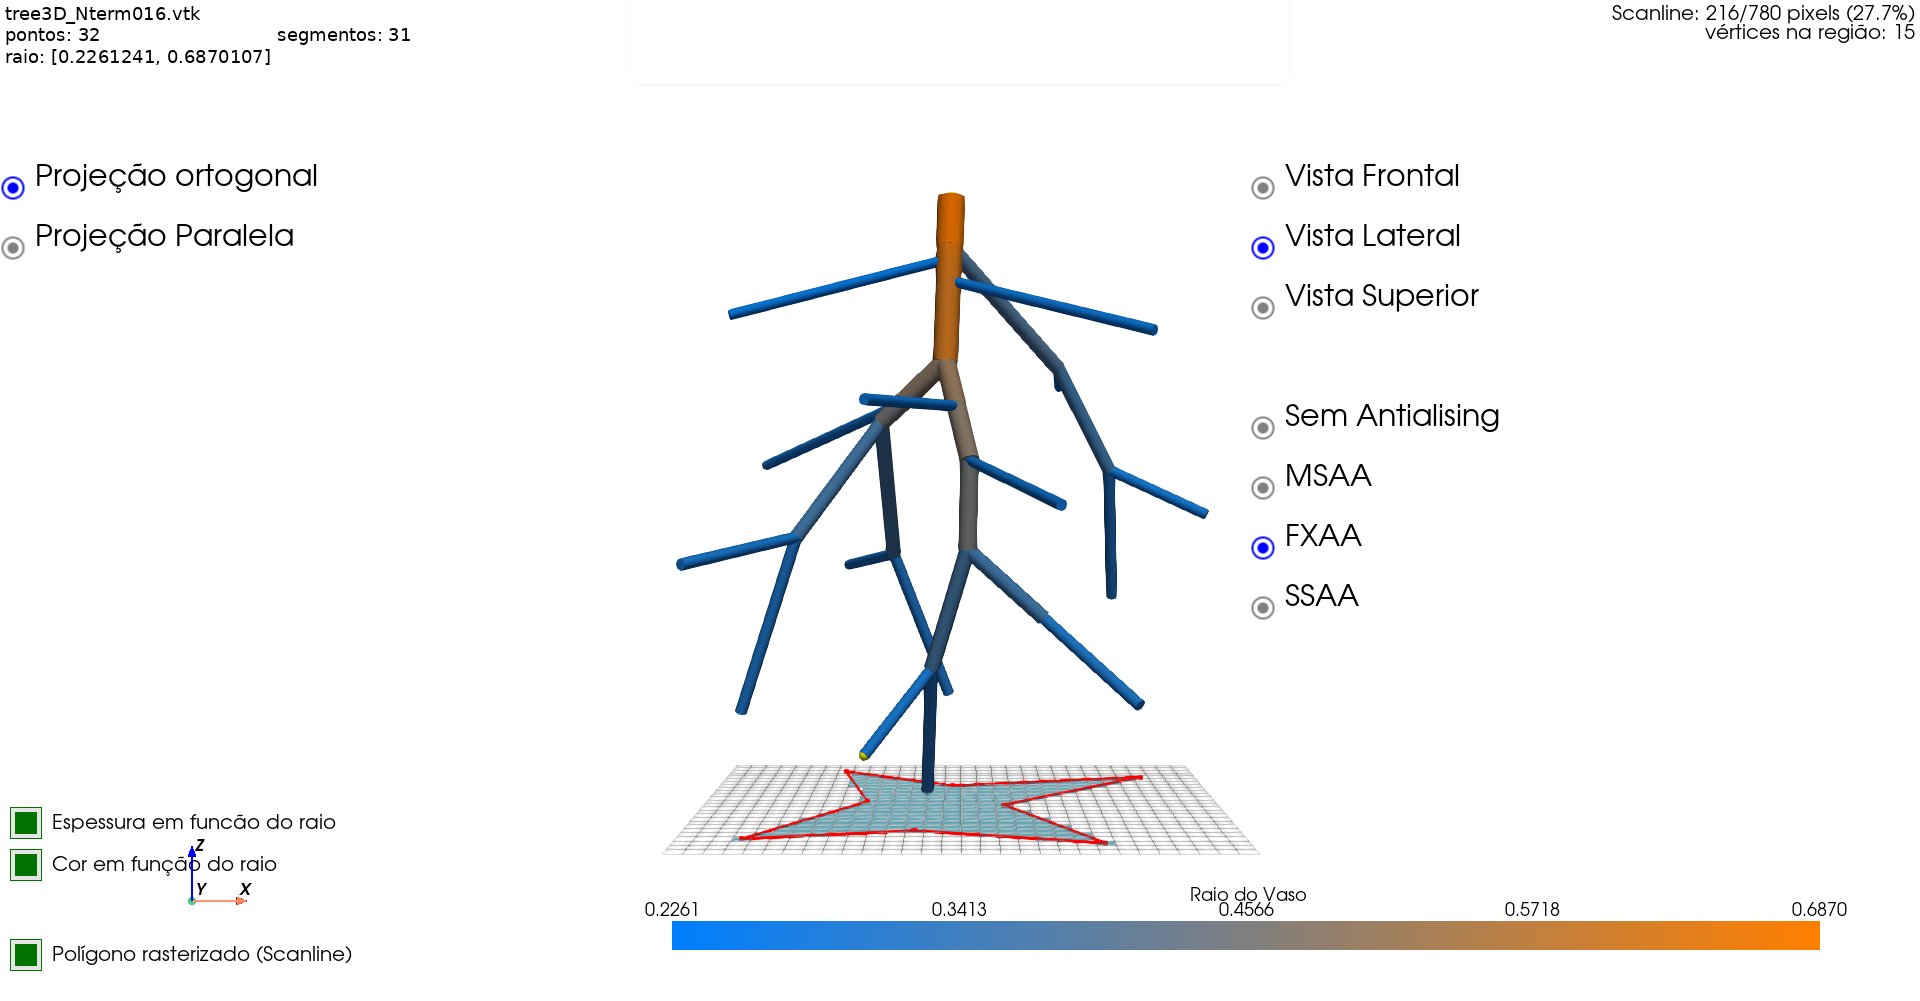
\includegraphics[width=\linewidth]{figures/aa_fxaa.png}
        \caption{FXAA.}
        \label{fig:fxaa}
    \end{subfigure}
    \hfill
    \begin{subfigure}{0.48\textwidth}
        \centering
        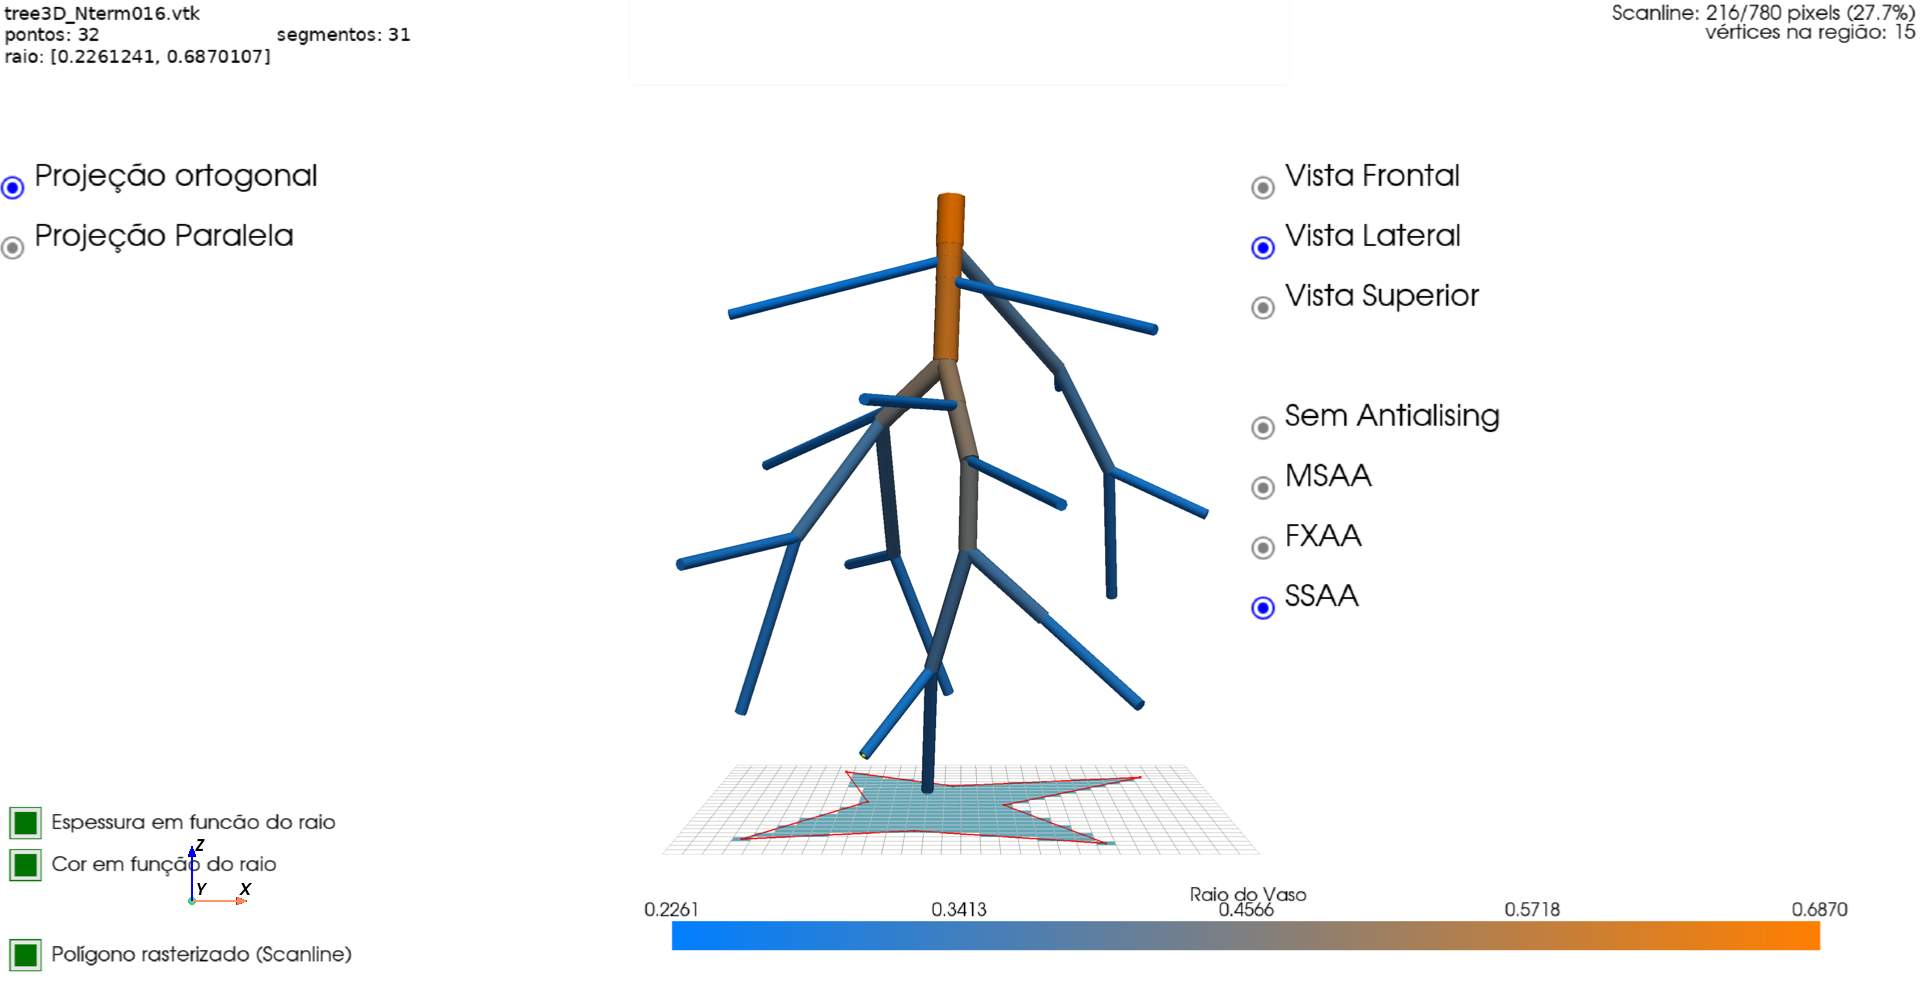
\includegraphics[width=\linewidth]{figures/aa_ssaa.png}
        \caption{SSAA.}
        \label{fig:ssaa}
    \end{subfigure}

    \caption{Comparação das diferentes configurações de Antialiasing.}
    \label{fig:comparacao_arvores_antiliasing}
\end{figure}

\subsection{Recorte de segmentos}

A Tabela~\ref{tab:clip} compara os algoritmos para a janela com fator de 50\% do tamanho da árvore para o modelo tree2D\_Nterm128.vtk. E a Figura \ref{fig:comparacao_recorte_linha} mostra visualmente a comparação da execução dos algoritmos.

\begin{table}[!h]
  \centering\small
  \caption{Estatísticas do recorte, obtidas dos contadores da aplicação.}
  \label{tab:clip}
  \begin{tabular}{|l|c|c|c|c|c|}
    \toprule
    \textbf{Algoritmo} & \textbf{Segmentos} & \textbf{Dentros} & \textbf{Cortados} & \textbf{Rejeitados} & \textbf{Interseções / Divisões} \\
    \midrule
    Cohen-Sutherland & 255 & 71 & 21 & 163 & 21 / 21\\
    Liang-Barsky & 255 & 53 & 39 & 163 & 0 / 733\\
    \bottomrule
  \end{tabular}
\end{table}

\begin{figure}[H]
    \centering
    \begin{subfigure}{0.48\textwidth}
        \centering
        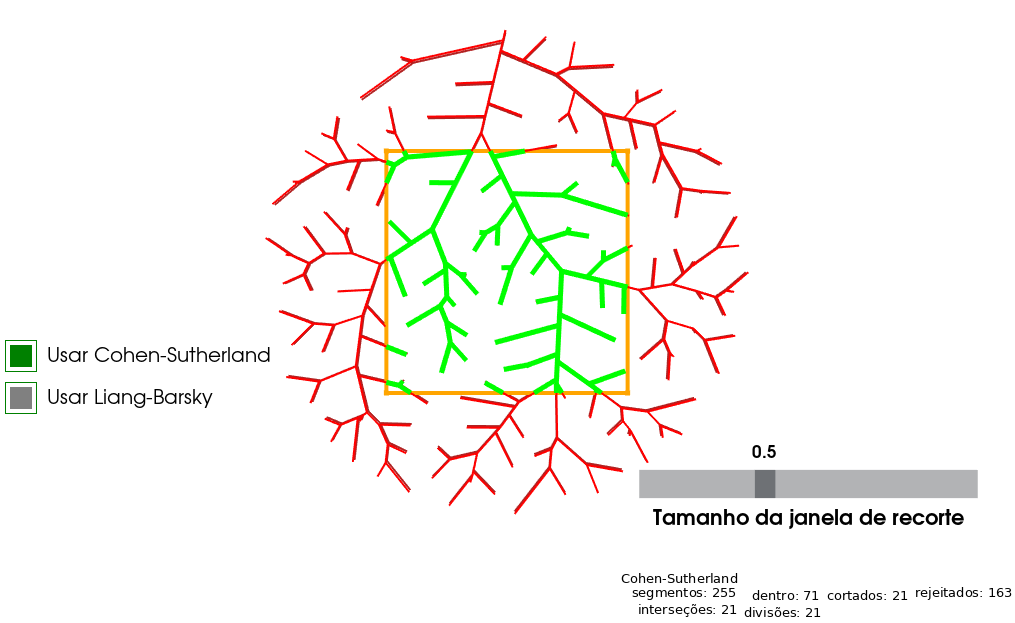
\includegraphics[width=\linewidth]{figures/cohen.png}
        \caption{Execução do algoritmo Cohen-Sutherland.}
        \label{fig:rasteriza2D}
    \end{subfigure}
    \hfill % Adiciona espaço horizontal entre as duas figuras
    \begin{subfigure}{0.48\textwidth}
        \centering
        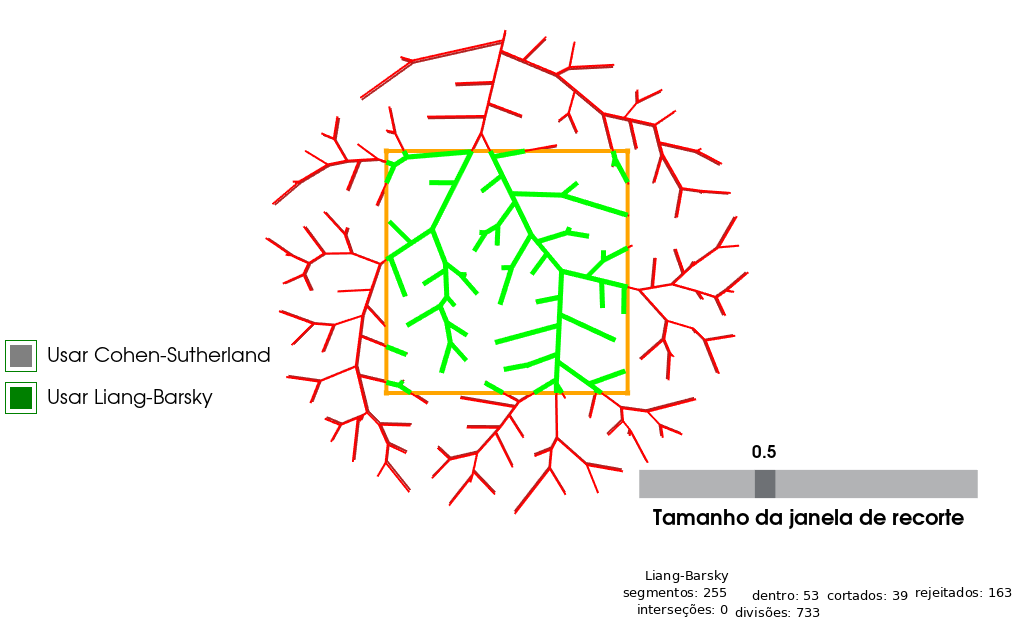
\includegraphics[width=\linewidth]{figures/liang.png}
        \caption{Execução do algoritmo Liang-Barsky.}
        \label{fig:rasteriza3D}
    \end{subfigure}

    \caption{Comparação da execução dos algoritmos Cohen-Sutherland e Liang-Barsky.}
    \label{fig:comparacao_recorte_linha}
\end{figure}

\subsection{Recorte de polígonos}

Na Figura \ref{fig:recortePoligono} mostra o resultado da execução do algoritmo Sutherland-Hodgamn no recorte de polígonos.

\begin{figure}[H]
    \centering
    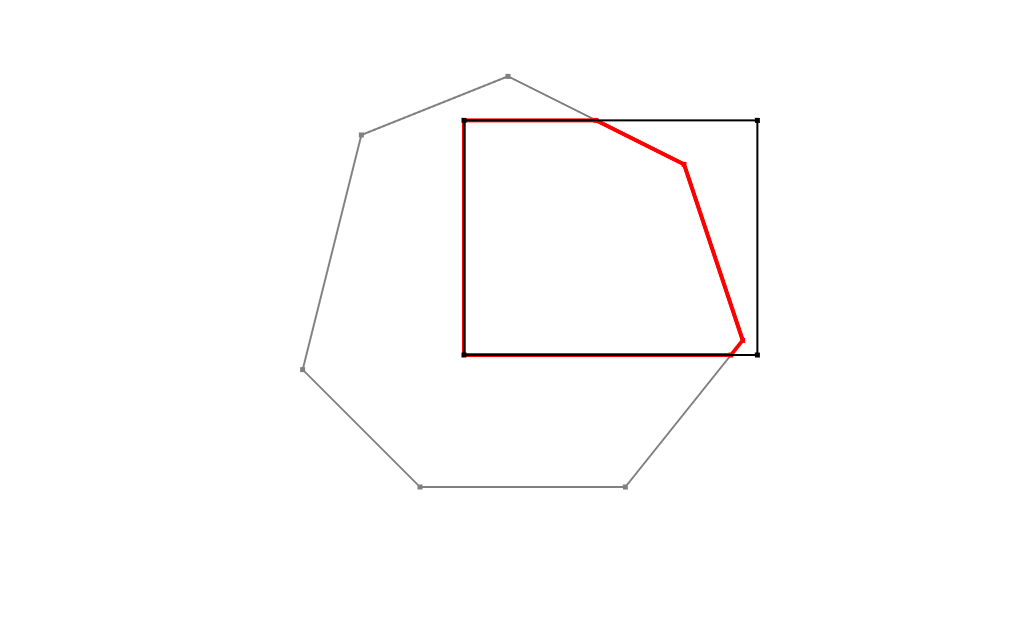
\includegraphics[width=0.75\linewidth]{figures/rasterizaçãoPoligoino.png}
    \caption{Recorte de Polígono.}
    \label{fig:recortePoligono}
\end{figure}

\section{Discussão}

Os resultados demonstram a integração de diferentes conceitos em uma aplicação única. O módulo 1 realiza a interpretação do arquivo VTK e constrói uma representação tubular que torna a estrutura vascular mais legível. A codificação do raio por cor e espessura amplia a quantidade de informação visual sem modificar a geometria topológica de entrada. O módulo 4 constitui a parte algorítmica mais explícita: o preenchimento é calculado em código próprio, com tabela de arestas e atualização incremental das interseções, em vez de ser delegado integralmente ao renderizador.

Há, entretanto, diferenças importantes entre os requisitos do enunciado e o estado atual do programa. O módulo 2 permite escolher vistas e alternar a projeção por meio da API, mas não implementa operações explícitas de translação, rotação e escala do objeto. A interface também apresenta os rótulos das projeções invertidos em relação às chamadas da câmera.


\subsection{Implementado pelo grupo × auxílio da biblioteca}
A Tabela~\ref{tab:atribuicao} separa explicitamente as partes.

\begin{table}[htbp]
  \centering\small
  \caption{Divisão entre o que foi implementado pelo grupo e o que foi fornecido pelo PyVista/VTK.}
  \label{tab:atribuicao}
  \begin{tabularx}{\textwidth}{l X X}
    \toprule
    \textbf{Tópico} & \textbf{Implementado pelo grupo} & \textbf{Auxílio de biblioteca}\\
    \midrule
    1. Leitura/atributos & Decomposição em segmentos, detecção do raio, mapa de cor, escala de espessura & Leitura do VTK; filtro de tubos\\
    2. Observador & Organização de vistas e botões & Câmera, matrizes de visão e projeção, interação\\
    3. Linhas & DDA e Bresenham & Figura com Matplotlib\\
    4. Polígonos & Scanline (ET/AET), geometria dos retângulos, projeção, rotação & Exibição do buffer como malha de pixels\\
    5. Antialiasing & Interface de seleção e comparação & MSAA, FXAA e SSAA\\
    6. Recorte de segmentos & Cohen-Sutherland, Liang-Barsky, interpolação de $z$, contadores & Exibição das linhas\\
    7. Recorte de polígonos & Sutherland-Hodgman (quatro bordas, histórico por etapa), polígono de teste, arraste da janela & Janela 2D, câmera paralela, eventos de mouse (VTK)\\
    \bottomrule
  \end{tabularx}
\end{table}

\subsection{Comparação entre os algoritmos de recorte}
Cohen-Sutherland é eficiente quando a maioria dos segmentos é trivialmente aceita ou rejeitada, mas, para segmentos que cruzam a janela, pode recalcular interseções e códigos por até quatro iterações, cada uma com uma divisão. Liang-Barsky calcula no máximo quatro razões $q_k/p_k$ e só obtém os pontos recortados uma vez ao final, evitando interseções intermediárias. Cyrus-Beck, não implementado, usa a mesma ideia paramétrica, mas aceita qualquer janela convexa, ao custo de produtos escalares em vez de simples diferenças de coordenadas.

\subsection{Sutherland-Hodgman e Weiler-Atherton}
Sutherland-Hodgman funciona com qualquer polígono contra uma janela convexa, mas, ao recortar polígonos côncavos, pode produzir arestas degeneradas (sobrepostas) ao ligar partes que deveriam ser regiões separadas, pois sua saída é sempre uma única lista de vértices. O Weiler-Atherton~\cite{weileratherton1977} é mais adequado quando há polígonos côncavos, quando a interseção gera múltiplas regiões disjuntas e quando a janela também é um polígono arbitrário, incluindo côncavo ou com buracos: ao percorrer as listas de entrada e saída, ele separa corretamente as regiões resultantes. Em contrapartida, é bem mais complexo de implementar.

\subsection{Decisões de implementação e limitações}
\begin{itemize}[leftmargin=*]
  \item O mapa de cores RGB linear é simples, mas não é perceptualmente uniforme; mapas contínuos como o \emph{viridis} facilitariam a leitura de diferenças sutis de raio.
  \item No DDA, a função \texttt{round} de Python arredonda valores intermediários ($x{,}5$) para o inteiro par mais próximo, o que pode gerar pequenas diferenças em relação ao Bresenham.
  \item O Módulo 3 rasteriza apenas os 20 primeiros segmentos, por clareza visual; a fração 500 de conversão para inteiros depende da escala do modelo.
  \item O recorte do Módulo 6 considera apenas o plano $xy$ (com interpolação de $z$); não há recorte volumétrico em 3D.
  \item No Módulo 4, a ordenação por profundidade é uma aproximação (algoritmo do pintor) e não substitui um Z-buffer.
  \item No Módulo 7, a janela só pode ser arrastada (tamanho fixo), a interface demonstra apenas o polígono convexo (o côncavo foi testado por chamada direta da função) e o módulo abre janela própria.
  \item O Sutherland-Hodgman implementado serve apenas a janelas retangulares alinhadas aos eixos e não separa regiões disjuntas.
\end{itemize}

\section{Conclusão}
Este trabalho resultou em uma aplicação modular que integra leitura, visualização, rasterização, antialiasing e recorte de modelos de árvores arteriais CCO. Os algoritmos clássicos solicitados (DDA e Bresenham, Scanline, Cohen-Sutherland, Liang-Barsky e Sutherland-Hodgman) foram implementados diretamente pelo grupo, enquanto a leitura dos arquivos, a renderização, a câmera e o antialiasing ficaram a cargo do PyVista/VTK, como documentado na Tabela~\ref{tab:atribuicao}.

Os experimentos permitiram observar, de forma concreta, o que os livros descrevem: DDA e Bresenham geram praticamente os mesmos pixels com custos diferentes; Cohen-Sutherland e Liang-Barsky recortam igualmente os segmentos, mas com quantidades distintas de interseções e divisões; e o Sutherland-Hodgman é simples e correto para polígonos convexos, mas não representa corretamente a saída quando o recorte de um polígono côncavo produz mais de uma região. O trabalho também deixou claro o contraste entre algoritmos didáticos e o pipeline gráfico, que realiza essas etapas em hardware.